% A LaTeX (non-official) template for ISAE projects reports
% Copyright (C) 2014 Damien Roque
%$ This program is free software; you can redistribute it and/or
% modify it under the terms of the GNU General Public License
% as published by the Free Software Foundation; either version 2
% of the License, or (at your option) any later version.

% This program is distributed in the hope that it will be useful,
% but WITHOUT ANY WARRANTY; without even the implied warranty of
% MERCHANTABILITY or FITNESS FOR A PARTICULAR PURPOSE.  See the
% GNU General Public License for more details.

% You should have received a copy of the GNU General Public License
% along with this program; if not, write to the Free Software
% Foundation, Inc., 51 Franklin Street, Fifth Floor, Boston, MA  02110-1301, USA.

% Version: 0.2
% Author: Damien Roque <damien.roque_AT_isae.fr>

\documentclass[a4paper,12pt]{report}
\usepackage[utf8]{inputenc}
\usepackage[T1]{fontenc}
\usepackage[french]{babel} % If you write in French
%\usepackage[english]{babel} % If you write in English
\usepackage{a4wide}
\usepackage{graphicx}
\graphicspath{{images/}}
\usepackage{subfig}
\usepackage{tikz}
\usetikzlibrary{shapes,arrows}
\usepackage{pgfplots}
\pgfplotsset{compat=newest}
\pgfplotsset{plot coordinates/math parser=false}
\newlength\figureheight
\newlength\figurewidth
\pgfkeys{/pgf/number format/.cd,
set decimal separator={,\!},
1000 sep={\,},
}
\usepackage{ifthen}
\usepackage{ifpdf}
\ifpdf
\usepackage[pdftex]{hyperref}
\else
\usepackage{hyperref}
\fi
\usepackage{color}
\hypersetup{%
colorlinks=true,
linkcolor=black,
citecolor=black,
urlcolor=black}

\renewcommand{\baselinestretch}{1.05}
\usepackage{fancyhdr}
\pagestyle{fancy}
\fancyfoot{}
\fancyhead[LE,RO]{\bfseries\thepage}
\fancyhead[RE]{\bfseries\nouppercase{\leftmark}}
\fancyhead[LO]{\bfseries\nouppercase{\rightmark}}
\setlength{\headheight}{15pt}

\let\headruleORIG\headrule
\renewcommand{\headrule}{\color{black} \headruleORIG}
\renewcommand{\headrulewidth}{1.0pt}
\usepackage{colortbl}
\arrayrulecolor{black}

\fancypagestyle{plain}{
  \fancyhead{}
  \fancyfoot[C]{\thepage}
  \renewcommand{\headrulewidth}{0pt}
}

\makeatletter
\def\@textbottom{\vskip \z@ \@plus 1pt}
\let\@texttop\relax
\makeatother

\makeatletter
\def\cleardoublepage{\clearpage\if@twoside \ifodd\c@page\else%
  \hbox{}%
  \thispagestyle{empty}%
  \newpage%
  \if@twocolumn\hbox{}\newpage\fi\fi\fi}
\makeatother
\graphicspath{{C:/Users/Utilisateur/Pictures/}  } %logo
\renewcommand{\thesection}{\alph{section}}
\usepackage{enumitem}
\usepackage{amsthm}
\usepackage{amssymb,amsmath,bbm}
\usepackage{array}
\usepackage{bm}
\usepackage{multirow}
\usepackage[footnote]{acronym}

\newcommand*{\SET}[1]  {\ensuremath{\mathbf{#1}}}
\newcommand*{\VEC}[1]  {\ensuremath{\boldsymbol{#1}}}
\newcommand*{\FAM}[1]  {\ensuremath{\boldsymbol{#1}}}
\newcommand*{\MAT}[1]  {\ensuremath{\boldsymbol{#1}}}
\newcommand*{\OP}[1]  {\ensuremath{\mathrm{#1}}}
\newcommand*{\NORM}[1]  {\ensuremath{\left\|#1\right\|}}
\newcommand*{\DPR}[2]  {\ensuremath{\left \langle #1,#2 \right \rangle}}
\newcommand*{\calbf}[1]  {\ensuremath{\boldsymbol{\mathcal{#1}}}}
\newcommand*{\shift}[1]  {\ensuremath{\boldsymbol{#1}}}

\newcommand{\eqdef}{\stackrel{\mathrm{def}}{=}}
\newcommand{\argmax}{\operatornamewithlimits{argmax}}
\newcommand{\argmin}{\operatornamewithlimits{argmin}}
\newcommand{\ud}{\, \mathrm{d}}
\newcommand{\vect}{\text{Vect}}
\newcommand{\sinc}{\ensuremath{\mathrm{sinc}}}
\newcommand{\esp}{\ensuremath{\mathbb{E}}}
\newcommand{\hilbert}{\ensuremath{\mathcal{H}}}
\newcommand{\fourier}{\ensuremath{\mathcal{F}}}
\newcommand{\sgn}{\text{sgn}}
\newcommand{\intTT}{\int_{-T}^{T}}
\newcommand{\intT}{\int_{-\frac{T}{2}}^{\frac{T}{2}}}
\newcommand{\intinf}{\int_{-\infty}^{+\infty}}
\newcommand{\Sh}{\ensuremath{\boldsymbol{S}}}
\newcommand{\C}{\SET{C}}
\newcommand{\R}{\SET{R}}
\newcommand{\Z}{\SET{Z}}
\newcommand{\N}{\SET{N}}
\newcommand{\K}{\SET{K}}
\newcommand{\reel}{\mathcal{R}}
\newcommand{\imag}{\mathcal{I}}
\newcommand{\cmnr}{c_{m,n}^\reel}
\newcommand{\cmni}{c_{m,n}^\imag}
\newcommand{\cnr}{c_{n}^\reel}
\newcommand{\cni}{c_{n}^\imag}
\newcommand{\tproto}{g}
\newcommand{\rproto}{\check{g}}
\newcommand{\LR}{\mathcal{L}_2(\SET{R})}
\newcommand{\LZ}{\ell_2(\SET{Z})}
\newcommand{\LZI}[1]{\ell_2(\SET{#1})}
\newcommand{\LZZ}{\ell_2(\SET{Z}^2)}
\newcommand{\diag}{\operatorname{diag}}
\newcommand{\noise}{z}
\newcommand{\Noise}{Z}
\newcommand{\filtnoise}{\zeta}
\newcommand{\tp}{g}
\newcommand{\rp}{\check{g}}
\newcommand{\TP}{G}
\newcommand{\RP}{\check{G}}
\newcommand{\dmin}{d_{\mathrm{min}}}
\newcommand{\Dmin}{D_{\mathrm{min}}}
\newcommand{\Image}{\ensuremath{\text{Im}}}
\newcommand{\Span}{\ensuremath{\text{Span}}}

\newtheoremstyle{break}
  {11pt}{11pt}%
  {\itshape}{}%
  {\bfseries}{}%
  {\newline}{}%
\theoremstyle{break}

%\theoremstyle{definition}
\newtheorem{definition}{Définition}[chapter]

%\theoremstyle{definition}
\newtheorem{theoreme}{Théorème}[chapter]

%\theoremstyle{remark}
\newtheorem{remarque}{Remarque}[chapter]

%\theoremstyle{plain}
\newtheorem{propriete}{Propriété}[chapter]
\newtheorem{exemple}{Exemple}[chapter]

\parskip=5pt
\sloppy

\begin{document}

%%%%%%%%%%%%%%%%%%
%%% First page %%%
%%%%%%%%%%%%%%%%%%

\begin{titlepage}
\begin{center}

\includegraphics[width=0.6\textwidth]{isae_logo.png}\\[1cm]

{\large Projet ingénieurie et entreprenariat 3A}\\[0.5cm]

%{\large Type de projet} \\[0.5cm]

% Title
\rule{\linewidth}{0.5mm} \\[0.4cm]
{\huge \bfseries Analyse de schémas numériques d'intégration temporelle \\[0.4cm] }
\rule{\linewidth}{0.5mm} \\[1.5cm]

% Author and supervisor
\noindent
\begin{minipage}{0.4\textwidth}
  \begin{flushleft} \large
    \emph{Auteurs :}\\
    M. Jean-Baptiste \textsc{Fourtout}\\
    M. Louis \textsc{Reboul}\\
    M\up{me} Sara \textsc{Barassa-Ramos}\\
    M. Pierre \textsc{Seize} \\
    M. Théo   \textsc{Maes}
  \end{flushleft}
\end{minipage}%
\begin{minipage}{0.4\textwidth}
  \begin{flushright} \large
    \emph{Encadrants :} \\
    Pr.~Xavier \textsc{Vasseur}\\
    Dr.~Guillaume \textsc{Puigt}
  \end{flushright}
\end{minipage}

\vfill

% Bottom of the page
%{\large Version 0.1 du \\  
\today
\end{center}
\end{titlepage}  

\tableofcontents
%\frontmatter

\chapter*{Introduction}
Ce document est rédigé dans le cadre du Projet Ingénieurie et Entrepreneuriat en dernière année de l'ISAE SUPAERO. Il s'agit ici d'analyser les performances de schémas numériques d’intégration
temporelle pour les simulations aux grandes échelles avec les méthodes spectrales discontinues d'ordre très élevé. Ces méthodes permettrait de pouvoir augmenter la pas de temps d'un calcul CFD. Et par conséquent semlbe très intéressant pour réduire les coûts de calcul.

Le travail effectué se base donc sur la publication de papier scientifique. Notre objectif est donc d'implémenter ces nouveaux types de schémas dit \og exponentiels \fg{} en langage python mais aussi d'en assurer le couplage avec les méthodes spatiales. 

\part{Gestion de projet}

\vfill

Cette partie consiste à exposer la manière dont nous nous sommes organisé pour la réalisation de ce projet. Ce sujet de PIE s'insrit globalement dans une stratégie commune de recherche entre l'ISAE-SUPAERO et l'ONERA. L'objectif est l'amélioration du code de calcul JAGUAR basé sur les différences spectrales ayant pour objectifs d'effectuer des simulations LES.


Les méthodes spectrales discontinues consistent à représenter la solution par cellule de calcul sur une base de polynôme et à prendre en compte la discontinuité entre cellules par résolution d’un problème de Riemann. Assez récentes en CFD, leur application pour là LES (SGE en Français) est un sujet de recherche actuel. Aujourd’hui, les études se focalisent essentiellement sur la précision des schémas spatiaux pour la convection et la diffusion. Ici, on souhaite focaliser notre attention sur les schémas numériques d’intégration temporelle des équations dans un code 1D prototype. Après une analyse bibliographique (Runge‐Kutta, Méthode de Gear, exponentiels, schémas Rock...), nous proposons d’implanter plusieurs familles de schémas dans une maquette 1D puis de comparer les schémas.

\vfill

\chapter{Description du projet}

\section{Objectifs du projet, périmètre et résultats attendus}
    Plusieurs résultats sont attendus : 
	\begin{itemize}[label=\textbullet,]
		\item Une analyse bibliographique des différentes classes de méthodes, 
		\item Une analyse théorique des schémas numériques (précision, cout algorithmique, CFL max...) avec prise en compte de leurs paramètres utilisateur 
		\item Une maquette (python) dans laquelle les schemas sont implantés (a gérer sous 
        GitHub) et plusieurs cas‐tests. 
		\item Un rapport sur la comparaison croisée des schémas numériques
		\item Une liste de recommandations du groupe sur le(s) meilleur (s) schéma(s)
	\end{itemize}
	
\section{Les parties prennantes du projet}	
   Il est important de bien connaître toutes les parties prenantes du projet afin que la communication entre les différentes parties soient fluides et efficace. 
   \begin{itemize}[label=\textbullet]
   	\item Groupe Etudiants de L’ISAE composé de Louis Reboul, Pierre Seize, Sara Barrasa-Ramos, Jean-Baptiste Fourtout, Maes Théo qui représente l’équipe de développeurs
   	\item Guillaume  Puigt pour l'Onera : Client et encadrant technique
   	\item Xavier Vasseur : Client, encadrant technique et référent école
   	\item Rémi Lebouteiller : Tuteur en gestion de projet
    \end{itemize}

\section{Les exigences de haut niveau}
    Les exigences client sont :
   \begin{itemize}[label=\textbullet]
   	\item Implémenter les méthodes numérique exponentielle Standard, Rosenbroch, Rock en 1D
   	\item Fournir et commenter le code
   	\item Donner les avantages et les inconvénients de chacune des méthodes afin de déterminer laquelle est la meilleur pour une utilisation souhaitée.
    \end{itemize}

\section{Les contraintes identifiées}
    Les contraintes connues à l’heure actuelle portent sur l’environnement de développement du logiciel, elles sont imposées par les clients :
   \begin{itemize}[label=\textbullet]
   	\item Utilisation du langage de programmation Python version 2.7.xx
   	\item Utilisation de la plateforme Github pour le partage des données
    \end{itemize}

\section{Hypothèses de travail}
    Les hypothèses du projet portent sur les ressources disponibles et la capacité de travail des membres de l’équipe de développement.
   \begin{itemize}[label=\textbullet]
   	\item L’équipe de développement peut fournir 4 à 8h/semaine/personne
   	\item Une partie de la bibliographie est fourni par G. Puigt et une autre par Xavier Vasseur
   	\item  Les algorithmes d’intégration spatiales sont fournis par G. Puigt
    \end{itemize}


\chapter{Organisation}
\section{Organisation de l’équipe (rôles)}
    Notre équipe est organisée de la manière suivante :
   \begin{itemize}[label=\textbullet]
   	\item Théo Maes sera notre chef de projet. 
   	\item {Nous avons divisé l’équipe en deux groupes opérationnels :
   	
   	    L’équipe développement, coordonnée par Sara Barrasa-Ramos, sera responsable de l'implémentation des méthodes numériques aux EDE. Elle sera composée de :
   	    \begin{itemize}[label=\textbullet]
   	    \item Louis Reboul
   	    \item Sara Barrasa-Ramos
   	    \item Théo Maes
        \end{itemize}
        
        L’équipe couplage, coordonnée par Pierre Seize, sera responsable de rendre compatible les schémas numériques d'intégration temporelle avec les schémas numériques d'intégration spatial existants . Elle sera composée de :
   	    \begin{itemize}[label=\textbullet]
   	    \item Pierre Seize
   	    \item Jean-Baptiste Fourtout
        \end{itemize}
        }
    \end{itemize}
\section{Organisation du travail (méthodes et outils)}
    C’est le diagramme OBS qui permet de donner sous forme de diagramme la hiérarchisation de notre projet.
    
    \begin{center}
		
    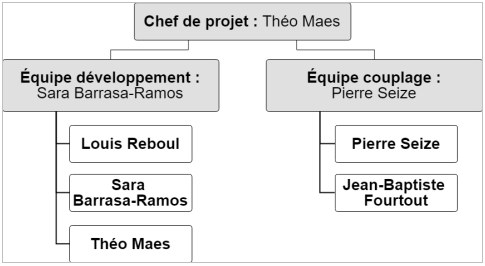
\includegraphics[width=1\textwidth]{images/OBS.png}\\[1cm]
    
    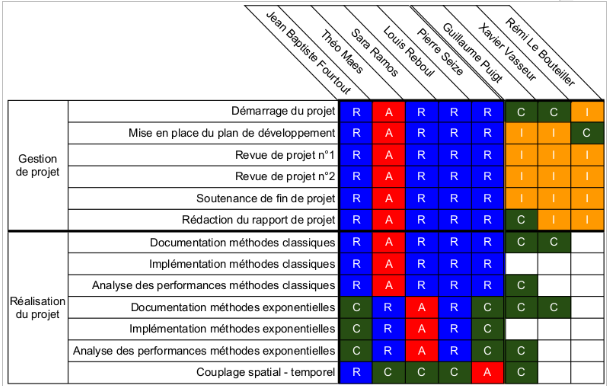
\includegraphics[width=1\textwidth]{images/OB2.png}\\[1cm]

    \end{center} 
    
\chapter{Processus du développement}
\section{Logique de développement}

    Nous avons commencé par prendre connaissance de la bibliographie qui est directement liée à notre travail. Puis il a fallu prendre en main la programmation Python car tous les développeurs n’avaient pas la même connaissance de ce langage informatique. L’Onera développe un logiciel de calcul CFD très performant, qui est limité par la capacité de résolution des méthodes temporelles. C’est pourquoi l’objectif de ce projet est d’améliorer les méthodes temporelles utilisées dans le code informatique. Il faut donc implémenter des méthodes dites « Exponentielles » qui sont récentes et seraient plus efficaces que les méthodes connues classique du type Range-Kutta. Afin de prendre en main la programmation nous avons coder les méthodes classiques afin de connaître leurs performances. Puis nous codons alors les méthodes exponentielles afin de pouvoir comparer les performances avec les méthodes classiques. Une fois ceci réalisé nous devons faire un choix sur la méthode que nous allons coupler avec la méthode de résolution spatiale pour la finalisation du logiciel de calcul de l’Onera. 

\section{Définition des jalons}

    Définition des jalons et la nature des jalons :
   \begin{itemize}[label=\textbullet]
   	\item 21/11/2018 : Première revue de projet à Présentation orale de l’avancée des travaux
   	\item 30/01/2018 : Deuxième revue de projet à Présentation orale de l’avancée des travaux plus début de rapport du projet
   	\item  Mi-Mars : Soutenance de projet à Présentation orale de l’ensemble du projet et des problèmes rencontrés
   	\item  Fin Mars : Livraison des livrables à Rapport de projet, Code source
    \end{itemize}

\section{Planning de projet (diagramme de Gantt)}

    \begin{center}

    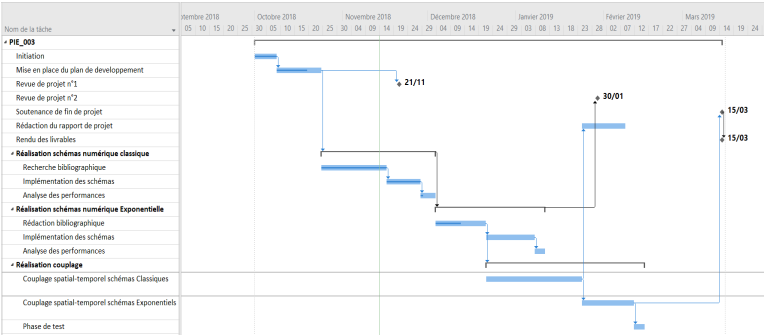
\includegraphics[width=1\textwidth]{images/Gant.png}\\[1cm]

    \end{center} 

\chapter{Definition détaillée du projet (Diagrammes PBS et WBS}

\begin{figure}
     \centering
      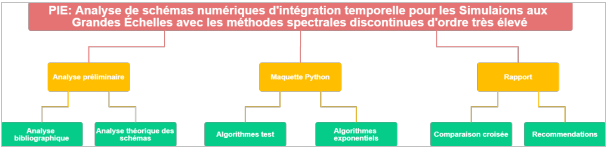
\includegraphics[width=0.7\textwidth]{images/PBS.png}
       \caption{Diagramme PBS}
    \label{chaine optim}
\end{figure}
    
  \begin{figure}
     \centering
       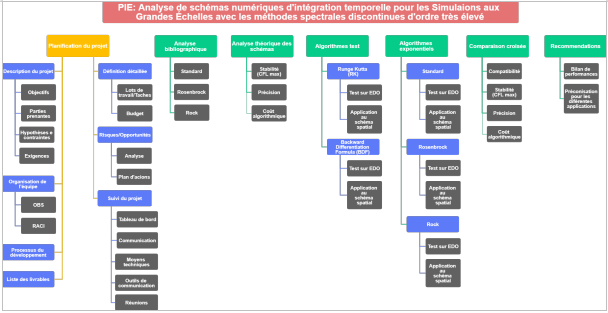
\includegraphics[width=0.7\textwidth]{images/WBS.png}
       \caption{Diagramme WBS}
     \label{chaine optim}
  \end{figure}
    
\chapter{Les livrables du projet}
\section{Liste des produits livrables au client}
   Les livrables du projet :
   \begin{itemize}[label=\textbullet]
   	\item Revue bibliographique avec pour objectif de répondre aux questions qu’est ce qu’on conseil d’utiliser et pourquoi ? Pour quelles applications ?
   	\item Compte rendu de projet sous format papier (ci-présent)
   	\item Rendu des supports utilisés pour la soutenance finale, très certainement un fichier Power Point
   	\item  Code informatique avec pour critère d’acceptation d’être fait en langage Python et transmis par la plateforme Github.
    \end{itemize}

\section{Liste des livrables demandés par l’école }

    Dans le cadre de la gestion de projet nous devons rendre un plan de développement de notre projet. D’autre part nous sommes évalués sur un rapport de projet et une soutenance qui aura lieu mi-Mars ce sont donc des livrables requis. 

\chapter{Risques et opportunités}

    \begin{center}

    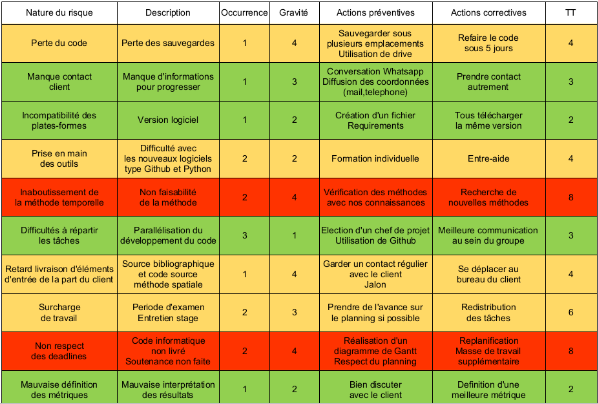
\includegraphics[width=1\textwidth]{images/matrice.png}\\[1cm]

    \end{center} 
    
\chapter{Suivi et Contrôle}
\section{Tableau de bord de suivi}
    Nous avons l’opportunité d’utiliser MS-Project pour faire un suivi du projet. Nous avons réalisé un diagramme de Gantt de référence que nous mettrons à jours au fur et à mesure que le projet va avancer. Nous savons déjà qu’en fin de projet des personnes sont en surcharge de travail, nous sommes déjà en train de voir comment nous allons pouvoir répartir la charge de travail. 

\section{Communication }

    Nous avons la chance d’avoir un de nos clients qui est très proche de nous, c’est pourquoi nous avons une conversation Whatsapp avec celui-ci. Mais notre référent école qui est aussi l’un de nos clients n’utilise pas cette interface c’est pourquoi pour dialoguer nous utilisons principalement les mails. C’est l’unique moyen de communication que nous avons d’ailleurs avec notre tuteur de gestion de projet. 
    
    D’autre part en moyenne nous avons décidé de faire des réunions bimensuelles ce qui permet rester à l’écoute de nos clients concernant leurs exigences qui peuvent évoluer au cours du temps. 
    
    Concernant la communication au sein de l’équipe nous avons un groupe sur le web de façon à partager et modifier facilement des documents sur lesquels nous travaillons. Une conversation téléphonique de groupe a été créée afin de se coordonner lors de réunions et de créneaux projet. 

\part{Méthodes numériques}
\chapter{Méthodes spectrales}
\section{Intérêt}
\section{Formalisme}
\section{Méthode de reconstitution du Flux}

\chapter{Méthodes temporelles}
\section{Exponentiel}
\section{Rosenbroch}

\part{Couplage spatial - temporel}
\clearpage
\listoffigures

\clearpage
\chapter*{Liste des sigles et acronymes}
\begin{acronym}[CP-OFDMX] % Give the longest acronym here
\acro{ASK}{\emph{Amplitude Shift Keying}}
\acro{AWGN}{\emph{Additive White Gaussian Noise}}
\acro{BABG}{Bruit Additif Blanc Gaussien}
\acro{BCJR}{\emph{Bahl, Cocke, Jelinek, Raviv}}
\acro{BER}{\emph{Binary Error Rate}}
\acro{BFDM}{\emph{Biorthogonal Frequency Division Multiplexing}}
\end{acronym}

%%%%%%%%%%%%%%%%%%%%%%%%%%%%%%%%%%%%%%%%%%%%
%%% Content of the report and references %%%
%%%%%%%%%%%%%%%%%%%%%%%%%%%%%%%%%%%%%%%%%%%%

%\mainmatter
%\pagestyle{fancy}

%\cleardoublepage

%\include{01-introduction}
%\include{02-first-chapter}
%\include{03-another-chapter}
%\include{04-conclusion}

%\appendix

%\bibliographystyle{authoryear-fr}
%\bibliography{references}

%\clearpage

%%%%%%%%%%%%%%%%
%%% Abstract %%%
%%%%%%%%%%%%%%%%

\thispagestyle{empty}

\vspace*{\fill}
\noindent\rule[2pt]{\textwidth}{0.5pt}\\
{\textbf{Résumé ---}}
Lorem ipsum dolor sit amet, consectetur adipiscing elit. Sed non risus. Suspendisse lectus tortor, dignissim sit amet, adipiscing nec, ultricies sed, dolor. Cras elementum ultrices diam. Maecenas ligula massa, varius a, semper congue, euismod non, mi. Proin porttitor, orci nec nonummy molestie, enim est eleifend mi, non fermentum diam nisl sit amet erat. Duis semper. Duis arcu massa, scelerisque vitae, consequat in, pretium a, enim. Pellentesque congue. Ut in risus volutpat libero pharetra tempor. Cras vestibulum bibendum augue. Praesent egestas leo in pede. Praesent blandit odio eu enim. Pellentesque sed dui ut augue blandit sodales. Vestibulum ante ipsum primis in faucibus orci luctus et ultrices posuere cubilia Curae; Aliquam nibh. Mauris ac mauris sed pede pellentesque fermentum. Maecenas adipiscing ante non diam sodales hendrerit. Ut velit mauris, egestas sed, gravida nec, ornare ut, mi. Aenean ut orci vel massa suscipit pulvinar. Nulla sollicitudin. Fusce varius, ligula non tempus aliquam, nunc turpis ullamcorper nibh, in tempus sapien eros vitae ligula. Pellentesque rhoncus nunc et augue. Integer id felis.

{\textbf{Mots clés :}}
Lorem ipsum dolor sit amet, consectetur adipiscing elit. Sed non risus. Suspendisse lectus tortor.
\\
\noindent\rule[2pt]{\textwidth}{0.5pt}
\begin{center}
  ISAE\\
  10, avenue Édouard Belin\\
  BP 54032\\
  31055 Toulouse CEDEX 4
\end{center}
\vspace*{\fill}

\end{document}